% ===========================================================================
% Figure: Sybil-k and laundering-r, protocol v2 option B, GPT-4o-mini answers,
% oracle audits, target-specific ASR (%), 24 groups.
% Source (read-only): research_data/protocol_v2_optionB_run_v1/analysis/analysis.json
%   cells sybil_k{1,2,4,8}, launder_r{0..4}, metric target_asr.value x 100
%   (one decimal; identical, after rounding, to analysis/tables.md Tables 3-4,
%   Panel A). Not drawn because they coincide with a drawn line: C = S under
%   Sybil (every k), C = M under laundering (every r), SL within 3.2 points
%   of S, RandEC = undefended. Requires pgfplots (compat 1.17).
% ===========================================================================
\begingroup
\definecolor{svS}{HTML}{5B4BB7}
\definecolor{svM}{HTML}{555555}
\definecolor{svID}{HTML}{C98A00}
\definecolor{svML}{HTML}{1F6FB2}
\definecolor{svAG}{HTML}{2E8B57}
\definecolor{svSan}{HTML}{8FB8DE}
\definecolor{svSt}{HTML}{C0392B}
\pgfplotsset{
  svax/.style={width=0.40\textwidth, height=3.9cm, ymin=-3, ymax=72,
    ytick={0,20,40,60}, grid=major, grid style={black!10},
    tick label style={font=\sffamily\scriptsize}, label style={font=\sffamily\scriptsize},
    title style={font=\sffamily\scriptsize\bfseries, yshift=-4pt},
    every axis plot/.append style={line width=0.9pt, mark size=1.4pt}},
}
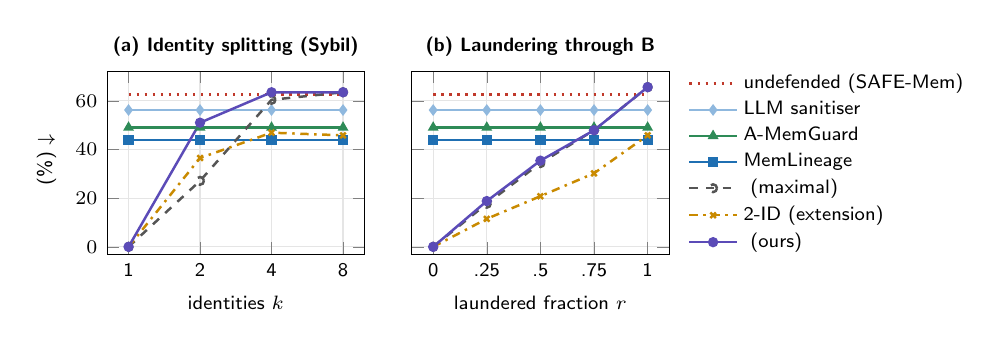
\begin{tikzpicture}
\begin{axis}[svax, name=left, title={(a) Identity splitting (Sybil)},
  xmode=log, log basis x=2, xtick={1,2,4,8}, xticklabels={1,2,4,8},
  xlabel={identities $k$}, ylabel={$\asrT$ (\%) $\downarrow$}]
\addplot[svSt, dotted, mark=none] coordinates {(1,62.5) (2,62.5) (4,62.5) (8,62.5)};
\addplot[svSan, mark=diamond*] coordinates {(1,56.2) (2,56.2) (4,56.2) (8,56.2)};
\addplot[svAG, mark=triangle*] coordinates {(1,49.0) (2,49.0) (4,49.0) (8,49.0)};
\addplot[svML, mark=square*] coordinates {(1,43.8) (2,43.8) (4,43.8) (8,43.8)};
\addplot[svM, dashed, mark=o] coordinates {(1,0.0) (2,27.1) (4,60.4) (8,63.5)};
\addplot[svID, dashdotted, mark=x] coordinates {(1,0.0) (2,36.5) (4,46.9) (8,45.8)};
\addplot[svS, mark=*] coordinates {(1,0.0) (2,51.0) (4,63.5) (8,63.5)};
\end{axis}
\begin{axis}[svax, at={(left.east)}, anchor=west, xshift=0.6cm,
  title={(b) Laundering through B},
  xtick={0,0.25,0.5,0.75,1}, xticklabels={0,.25,.5,.75,1},
  xlabel={laundered fraction $r$}, yticklabels={},
  legend style={at={(1.04,0.5)}, anchor=west, font=\sffamily\scriptsize, draw=none, fill=none, row sep=-1pt},
  legend cell align=left]
\addplot[svSt, dotted, mark=none] coordinates {(0,62.5) (0.25,62.5) (0.5,62.5) (0.75,62.5) (1,62.5)};
\addlegendentry{undefended (SAFE-Mem)}
\addplot[svSan, mark=diamond*] coordinates {(0,56.2) (0.25,56.2) (0.5,56.2) (0.75,56.2) (1,56.2)};
\addlegendentry{LLM sanitiser}
\addplot[svAG, mark=triangle*] coordinates {(0,49.0) (0.25,49.0) (0.5,49.0) (0.75,49.0) (1,49.0)};
\addlegendentry{A-MemGuard}
\addplot[svML, mark=square*] coordinates {(0,43.8) (0.25,43.8) (0.5,43.8) (0.75,43.8) (1,43.8)};
\addlegendentry{MemLineage}
\addplot[svM, dashed, mark=o] coordinates {(0,0.0) (0.25,17.7) (0.5,34.4) (0.75,47.9) (1,65.6)};
\addlegendentry{\armM{} (maximal)}
\addplot[svID, dashdotted, mark=x] coordinates {(0,0.0) (0.25,11.5) (0.5,20.8) (0.75,30.2) (1,45.8)};
\addlegendentry{\armS{}2-ID (extension)}
\addplot[svS, mark=*] coordinates {(0,0.0) (0.25,18.8) (0.5,35.4) (0.75,47.9) (1,65.6)};
\addlegendentry{\armS{} (ours)}
\end{axis}
\end{tikzpicture}
\endgroup
